
%Satzcounter = 3
\begin{Satz}[verallgemeinerter Mittelwertsatz]{
	\label{satz_9}
	Seien $f,g : [a,b] \rightarrow \mathbb{R}$ stetig und auf ganz 
	$\left( a, b \right)$ differenzierbar. Dann existiert ein 
	$\xi \in (a,b) $ mit:
	\begin{align*}
		\left( g(b)- g(a)\right)f'(\xi) = 
		\left( f(b) - f(a) \right) g'(\xi)
	\end{align*}
	\textbf{Beweis:} Wir betrachten $h: [a,b] \rightarrow \mathbb{R}$ 
	\begin{align*}
		t \mapsto \left( g(b) -g(a)\right)f(t) - \left(f(b)-f(a)\right)g(t)
	\end{align*}
	Offensichtlich \textit{(nach Summenregel)} ist $h$ differenzierbar auf $(a,b)$.
	Es gilt:
	\begin{align*}
		h'(t) = \left(g(b)-g(a)\right)f'(t) - \left(f(b)-f(a)\right)g'(t)
	\end{align*}
	Wir zeigen: es existiert ein $\xi \in (a,b)$ mit $h'(\xi) = 0$. Damit folgt 
	dann die Aussage. \\
	\textbf{Beachte:} 
	\begin{align*}
		h(a) = & \left(g(b)-g(a)\right)f(a) - \left(f(b)-f(a)\right)g(a) \\
		= & g(b) \cdot f(a) - f(b) \cdot g(a) \\
		= & \left(g(b) - g(a)\right)f(b) - \left(f(b)-f(a)\right)g(b) \\
		= & h(b)
	\end{align*}
	\textbf{Fall 1:}$h = const$ Dann gilt trivialerweise $h' = 0$ 
	und wir sind fertig. \\
	\textbf{Fall 2:}$h \neq const$ Offensichtlich ist $h$ stetig auf dem 
	abgeschlossenen Intervall $[a,b]$. Damit besitzt $h$ ein globales Maximum und 
	ein globales Minimum. Ohne Einschränkung existiert ein $\tilde{\xi} \in (a,b)$
	 mit $h(\tilde{\xi}) > h(a)$, sonst betrachte $-h$ statt $h$. \\
	 Also existiert ein $\xi \in (a,b)$ mit $h(\xi) \geq h(x)\textbf{ }
	  (x \in [a,b])$. 
	 Mit anderen Worten: $\xi$ ist auch ein globales Maximum und und daher auch 
	 ein lokales Maximum. Mit Satz~\ref{satz_8}
	 folgt: $h'(\xi) = 0$
	 \begin{figure}[h]
\centering
	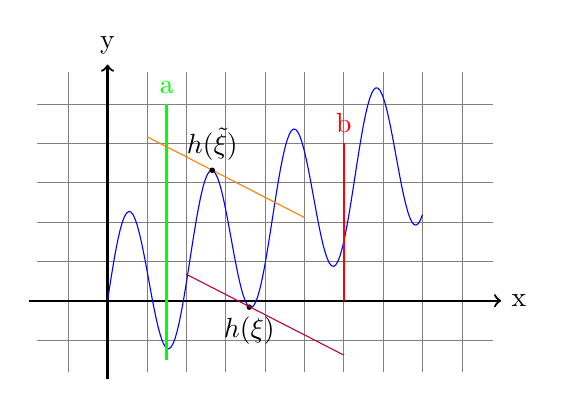
\begin{tikzpicture}
		\draw[very thin, gray, step = 0.5] (-0.9,-0.9) grid (4.9,2.9);
		\draw[->,thick, black](-1,0) -- (5,0) node[right]{x};
		\draw[->,thick, black](0,-1) -- (0,3) node[above]{y};
		\draw[blue,domain = 0.0:4.0, samples=150]   
			plot (\x,{(sin(6*\x r))+ 0.5*\x});
       	\draw[green,thick](0.75,-0.75)--(0.75,2.5)node[above]{a};
       	\draw[red,thick](3,0) -- (3,2) node[above]{b};
       	\draw[black](1.33,2.34079);
       	\draw[orange,domain = 0.5:2.5, samples = 150]
       		plot(\x,-0.5133*\x+2.3407);
       	\fill[black](1.33,1.657)circle(1pt)node[above]{$h(\tilde{\xi})$};
       	\fill[black](1.8,-0.0809)circle(1pt)node[below]{$h(\xi)$};
       	\draw[purple,domain = 1:3, samples = 150]
       		plot(\x,-0.5133*\x+0.85);
	\end{tikzpicture}
\end{figure}
}\end{Satz}
	
\begin{Satz}[Mittelwertsatz(MWS)]{\label{vl_07_MWS}
	Sei $f: [a,b] \rightarrow \mathbb{R}$ stetig und differenzierbar auf 
	(a,b). Dann gibt ex ein $\xi \in (a,b)$ mit 
	\begin{align*}
		f(b) -f(a) = (b-a) \cdot f'(\xi)
	\end{align*}
	\textbf{Bemerkung:} Es ist oft wichtig, dass f nur auf $(a,b)$ differenzierbar 
	sein muss. \\
	\textbf{Beweis:} Das folgt aus Satz~\ref{satz_9}
	mit $g = id_{[a,b]}$, d.h. $g(x) = x \textbf{ } (x \in [a,b])$.
}\end{Satz}

\begin{Satz}{
	\label{satz_11}
	Sei $f:[a,b] \rightarrow \mathbb{R}$ stetig und differenzierbar auf $(a,b)$. 
	Dann gilt:
	\renewcommand{\labelenumi}{\alph{enumi})}
	\begin{enumerate}
		\item $f = const \Leftrightarrow f'(x) = 0 (x\in(a,b))$
		\item $f$ ist monoton wachsend $\Leftrightarrow f'(x) \geq 0 (x \in (a,b))$
		\item $f$ ist streng monoton wachsend $\Leftrightarrow f'(x) > 0 (x \in (a,b
		))$
		\item $f$ ist monoton fallend $\Leftrightarrow f'(x) \leq 0 (x \in (a,b))$
		\item $f$ ist streng monoton fallend $\Leftrightarrow f'(x) < 0 
		(x \in (a,b))$ 
	\end{enumerate}
	\textbf{Beweis:} a) folgt aus b) und c). \\
	Weiterhin folgt d) beziehungsweise e) aus b) beziehungsweise c). \\
	Sei $ y > x \in [a,b]$. Sei $f|_{[x,y]}$ die \textit{Einschränkung} 
	von f auf $[x,y]$, das heißt: 
	\begin{equation*}
		f|_{[x,y]} : [x,y] \rightarrow \mathbb{R}, z \mapsto f(z)
	\end{equation*}
	Offensichtlich erfüllt $f|_{[x,y]}$ die Bedingungen des MWS. \\
	Es existiert 
	ein $\xi \in (x,y)$ mit $f(y)-f(x) = (y-x)\cdot f'(\xi)$\\
	\textbf{Fall b)} $f(y)-f(x) = (y-x)\cdot f'(\xi) \geq 0$ \\
	\hspace*{1.5cm}\rotatebox[origin=c]{180}{$\Lsh$} $f(y) \geq f(x) $ \\
	\textbf{Fall c)} $f(y)-f(x) > 0$ \\
	\hspace*{1.5cm}\rotatebox[origin=c]{180}{$\Lsh$}$f(y) > f(x)$ \\
	\textbf{Beweis der Richtung $\Leftarrow$ in Teil b):} Ist $f'(x) \geq 0$ so gilt
	\begin{align*}
		\lim\limits_{y \searrow x}{\frac{f(y)-f(x)}{y-x}}
		=\lim\limits_{y \nearrow x}{\frac{f(x) -f(y)}{x-y}} \geq 0
	\end{align*}
	Da $f$ monoton wachsend ist, gilt für $y > x$: 
	\begin{align*}
		\frac{f(y)-f(x)}{y-x} \geq 0
	\end{align*}	 
	Folglich gilt: 
	\begin{align*}
		\lim\limits_{y \searrow x}{\frac{f(y)-f(x)}{y-x} } \geq 0
	\end{align*}
	Äquivalent für $\lim\limits_{y \nearrow x}{ }$ 
}\end{Satz}


\begin{Korollar}{
	Seien $f,g : [a,b] \rightarrow \mathbb{R}$ stetig und differenzierbar auf
	$(a,b)$ mit $f'(x) = g'(x)$ für $x \in (a,b)$. Dann gilt $f-g = const$\\
	\textbf{Beweis:} Es gilt: 
	\begin{align*}
		(f-g)'(x) = f'(x)-g'(x) = 0
	\end{align*}
	Damit folgt die Aussage mit Satz~\ref{satz_11}.
}\end{Korollar}

\begin{Satz}{
	Sei $f: I \rightarrow \mathbb{R}$ zweimal differenzierbar $(I \subseteq 
	\mathbb{R}$ Intervall$)$. Gibt es $\xi \in I$ mit $f'(\xi) = 0$ und 
	$f''(\xi) < 0 \textbf{ }  (f''(\xi)> 0)$, so nimmt $f$ an der Stelle $\xi$ ein 
	striktes lokales Maximum (Minimum) an.\\
	\textbf{Beweis:} Wir betrachten nur den Fall $f''(\xi) < 0$. Für den Fall
	$f''(\xi) > 0$ betrachte man $-f$.\\
	Per Definition haben wir also: 
	\begin{align*}
		f''(\xi) = \lim\limits_{x \rightarrow \xi}{\frac{f'(x) - f'(\xi)}{x - \xi} }
		< 0
	\end{align*}
	$r := \lim\limits_{x \rightarrow \xi}{\frac{f'(x) - f'(\xi)}{x - \xi} } $ \\
	D.h. es existiert für jedes $ \epsilon > 0$ ein $\delta > 0$ mit
	\begin{align*}
		\left\vert \frac{f'(x) - f'(\xi)}{x - \xi} - r \right\vert < \epsilon
	\end{align*}
	
	Für $\epsilon := \frac{r}{2}$ gilt daher: 
	\begin{align*}
		\left\vert \frac{f'(\xi) - f'(x)}{\xi - x}-r \right\vert < \left\vert \frac{r}{2} \right\vert
	\end{align*}
	für ein entsprechend gewähltes $\delta > 0$. Insbesondere gilt also:
	\begin{align*}
		\frac{f'(\xi)-f'(x)}{\xi - x} < 0
	\end{align*}
	für alle $ x \in ( \xi - \delta, \xi + \delta)$.\\
	D.h. für $x < \xi$ gilt: 
	\begin{align*}
		f'(\xi) - f'(x) < 0
	\end{align*}
	und für $ x > \xi$ gilt: 
	\begin{align*}
		f'(\xi) - f'(x) > 0
	\end{align*}
	Ergo: $f'$ ist streng monoton fallend auf $(\xi - \delta, \xi]$ und 
	streng monoton wachsend auf $[ \xi, \xi + \delta)$ \\
	Da $f'(\xi) = 0$ folgt, dass $f'(x) > 0$ für $x \in (\xi-\delta, \xi]$
	und $f'(x) <0 $ für $x \in [\xi, \xi + \delta)$.\\
	  Mit Satz~\ref{satz_11} folgt: \\
	  	\hspace*{5mm}$f|_{(\xi-\delta, \xi]}$ ist streng monoton wachsend und \\
	  	\hspace*{5mm}$f|_{[\xi, \xi + \delta)}$ ist streng monoton fallend.
}\end{Satz}

\begin{Satz}[Regel von l'Hospital]{
	Seien $f,g: (a,b) \rightarrow \mathbb{R}$ mit
	\begin{align*}
		-\infty \leq a < b \leq \infty
	\end{align*}		
	differenzierbar und $g'(x) \neq 0$ für alle $x \in (a,b)$. Weiter gelte:
	\begin{align*}
		\lim\limits_{x \rightarrow a}{\frac{f'(x)}{g'(x)} } = A
	\end{align*}
	Wobei  $ -\infty \leq A \leq \infty$ sei und 
	$\lim\limits_{x \rightarrow a}{f(x) = 0}$, \\ 
	sowie 
	$\lim\limits_{x \rightarrow a}{g(x) = 0} $
	bzw. $\lim\limits_{x\rightarrow a}{g(x) = \pm \infty}$.\\
	Dann gilt: $\lim\limits_{x \rightarrow a}{\frac{f(x)}{g(x)} = A}$.
	Die analoge Aussage gilt auch für $x \rightarrow b$.\\
	\textbf{Bemerkung:}
	\begin{itemize}
		\item Wir verwenden hier den erweiterten Grenzwertbegriff, d.h. $\pm \infty$ 
		sind als Grenzwerte zulässig.
		\item Zwei wesentliche Voraussetzungen:
			\begin{enumerate}
				\item $\lim\limits_{x \rightarrow a}
				{\frac{f'(x)}{g'(x)}}$ existiert!
				\item ebenso ist essentiell, dass $f,g \rightarrow 
				\frac{\circ }{\pm \infty}$
			\end{enumerate}
		\item Gegebenenfalls lässt sich l'Hospital iterieren:
		\begin{align*}
			\lim\limits_{x \rightarrow \infty}{\frac{x^2}{exp(x)}} = 
			\lim\limits_{x \rightarrow \infty}{\frac{2x}{exp(x)}} = 
			\lim\limits_{x \rightarrow \infty}{\frac{2}{exp(x)}} = 0
		\end{align*}
		\item Man kann l'Hospital auch verwenden um Ausdrücke der Form 
		$0 \cdot \infty$ zu behandeln, indem wir diese in die Form
		\begin{align*}
		 	\frac{\infty}{\infty} = \frac{\infty}{\frac{1}{\infty}}
		\end{align*}
		bzw. 
		\begin{align*}
			\frac{0}{0} = \frac{0}{\frac{1}{\infty}}
		\end{align*}
		umrechnen.
	\end{itemize}
	
	\textbf{Beweis:} Wir beschränken uns auf den Fall $x \rightarrow a$ 
	$(x \rightarrow b$ läuft analog$)$ und zeigen zunächst folgende Aussage: \\
	\textbf{Behauptung:} Sei $A \in [-\infty, \infty)$. \\ 
	Dann existiert für jedes $q > A$ ein $c > a$ mit $\frac{f(x)}{g(x)} < q$ $(x\in (a,c))$. \\
	\textbf{Beweis der Behauptung:} \\
	Da $\frac{f'(x)}{g'(x)} \overset{x \searrow a}{\rightarrow} A$ 
	existiert ein $c' > a$ mit: $\frac{f'(x)}{g'(x)}<r$ für ein beliebiges 
	$r \in (A,q)$ und $x \in (a,c')$.\\
	Nach dem verallgemeinerten Mittelwertsatz gilt:
	\begin{align}
		\label{gleichung_beweis_lh_1}
		\frac{f(x)-f(y)}{g(x)-g(y)} = \frac{f'(t)}{g'(t)}
	\end{align}
	für ein geeignetes $t$ zwischen $x$ und $y$. \\
	Für $a < x < y <c'$ gilt daher:
	\begin{align}
		\label{gleichung_beweis_lh_2}
		\frac{f(x)-f(y)}{g(x)-g(y)} < r
	\end{align}
	\begin{itemize}
		\item[Fall 1:] $f,g \overset{x \rightarrow a}{\rightarrow} 0$. 
		Nach Gleichung~\eqref{gleichung_beweis_lh_2}
		gilt für $x \rightarrow a$ 
		\begin{align*}
			\frac{-f(y)}{-g(y)} = \frac{f(y)}{g(y)} < r <q (y \in (a, c'))
		\end{align*}
		\item[Fall 2:] $g(x) \overset{x \rightarrow a}{\rightarrow}\pm \infty$
		Multipliziere \eqref{gleichung_beweis_lh_1} mit
		$\frac{g(x)-g(y)}{g(x)}$. \\
		Dann erhalten wir:
		\begin{align*}
			\frac{f(x)}{g(x)} - \frac{f(y)}{g(x)} = \frac{f'(t)}{g'(t)}
			\left( 1 - \frac{g(y)}{g(x)}\right) \\
			 \rightarrow \frac{f(x)}{g(x)} = \frac{f'(t)}{g'(t)} \left(
			1- \frac{g(y)}{g(x)}\right) + \frac{f(y)}{g(x)}
		\end{align*}
		Für $x \rightarrow a$:
		\begin{align*}
			\lim\limits_{x\rightarrow a}{\frac{f(x)}{g(x)}}\leq r < q
		\end{align*}
		Es muss also ein $ c > a$ existieren mit: 
		$\frac{f(x)}{g(x)} <r$ $(x \in (a,c))$ \\
		Analog kann man zeigen: \\
		\textbf{Behauptung' :} Sei $A  \in (-\infty, \infty]$. Dann existiert für 
		jedes $p <A$ ein $d > a$, so dass $p < \frac{f(x)}{g(x)}$ $(x \in (a,d))$\\
		Für $A = +\infty$ folgt die Aussage aus der letzten Behauptung, für 
		$ A = - \infty$ aus der ersten Behauptung. \\
		Für $A \in \mathbb{R}$ argumentieren wir wie folgt: \\
		Sei $\epsilon > 0$ gegeben. Nach der ersten Behauptung existiert 
		$c > a$, so dass $\frac{f(x)}{g(x)} < A + \epsilon$ $(x\in (a,c))$. 
		Nach der zweiten Behauptung existiert $d > a$ mit:
		\begin{align*}
			\frac{f(x)}{g(x)} > A - \epsilon \text{ } (x \in (a,d))
		\end{align*}
		Für $x \in (a, \min\{c,d\})$ gilt daher
		\begin{align*}
			\frac{f(x)}{g(x)} \in B_{\epsilon}(A)
		\end{align*}
	\end{itemize}	
	
}\end{Satz}

\begin{Beispiel}{
	$f(x) = 1, g(x) = x + 7$\\
	Dann gilt $\lim\limits_{x \rightarrow 0 }{\frac{f(x)}{g(x)} = \frac{1}{7}}$ \\
 aber:$ \lim\limits_{x \rightarrow 0 }{\frac{f'(x)}{g'(x)} = \frac{0}{	1}= 0}$
}\end{Beispiel}
